\chapter{كيمياء الحلقات غير المتجانسة}\label{ch:b3:heterocycles}

يحوي فنجان القهوة الكافيين، المبني من حلقتين ملتحمتين فيهما أربع
ذرات نيتروجين، وتأتي رائحتها من عشرات الفيورانات والبيرولات والبيرازينات
والثيوفينات المتكوّنة في أثناء التحميص. ومعظم الأدوية على رف الصيدلية تحوي
حلقة واحدة على الأقل فيها ذرة نيتروجين أو أكسجين أو كبريت، وكذلك قواعد
الحمض النووي، \omterm{def:b3:bioinorganic:haem}{والهيم} والكلوروفيل، وفيتامينات كثيرة. ويفسّر هذا الفصل كيف
تغيّر الذرة غير المتجانسة في حلقة عطرية إلكتروناتها: فقد تجعل الحلقة
أفقر من البنزين أو أغنى منه، وهذا يحدد أين تتفاعل وكيف. 
وينتهي بثلاث طرق كلاسيكية لبناء مثل هذه الحلقات.

\begin{recall}
عالج مجلد السنة الثانية العطرية وقاعدة هوكل، والأرينات 
والاستبدال العطري المحب للإلكترونات عبر وسيط ويلاند، والمجموعات
المنشِّطة والموجِّهة، والأمينات وقاعديتها، والإيمينات، والإينامينات،
والمتصاوغات والقواعد النووية؛ وعالج مجلد السنة الأولى $\mathrm pK_a$، والمحبات للنواة، 
والمحبات للإلكترونات والمجموعات المغادرة. وأعطى \cref{ch:b3:pericyclic} \omterm{def:b3:pericyclic:families}{إعادة الترتيب السيغماتروبية}
[3,3].
\end{recall}

\begin{omfigure}
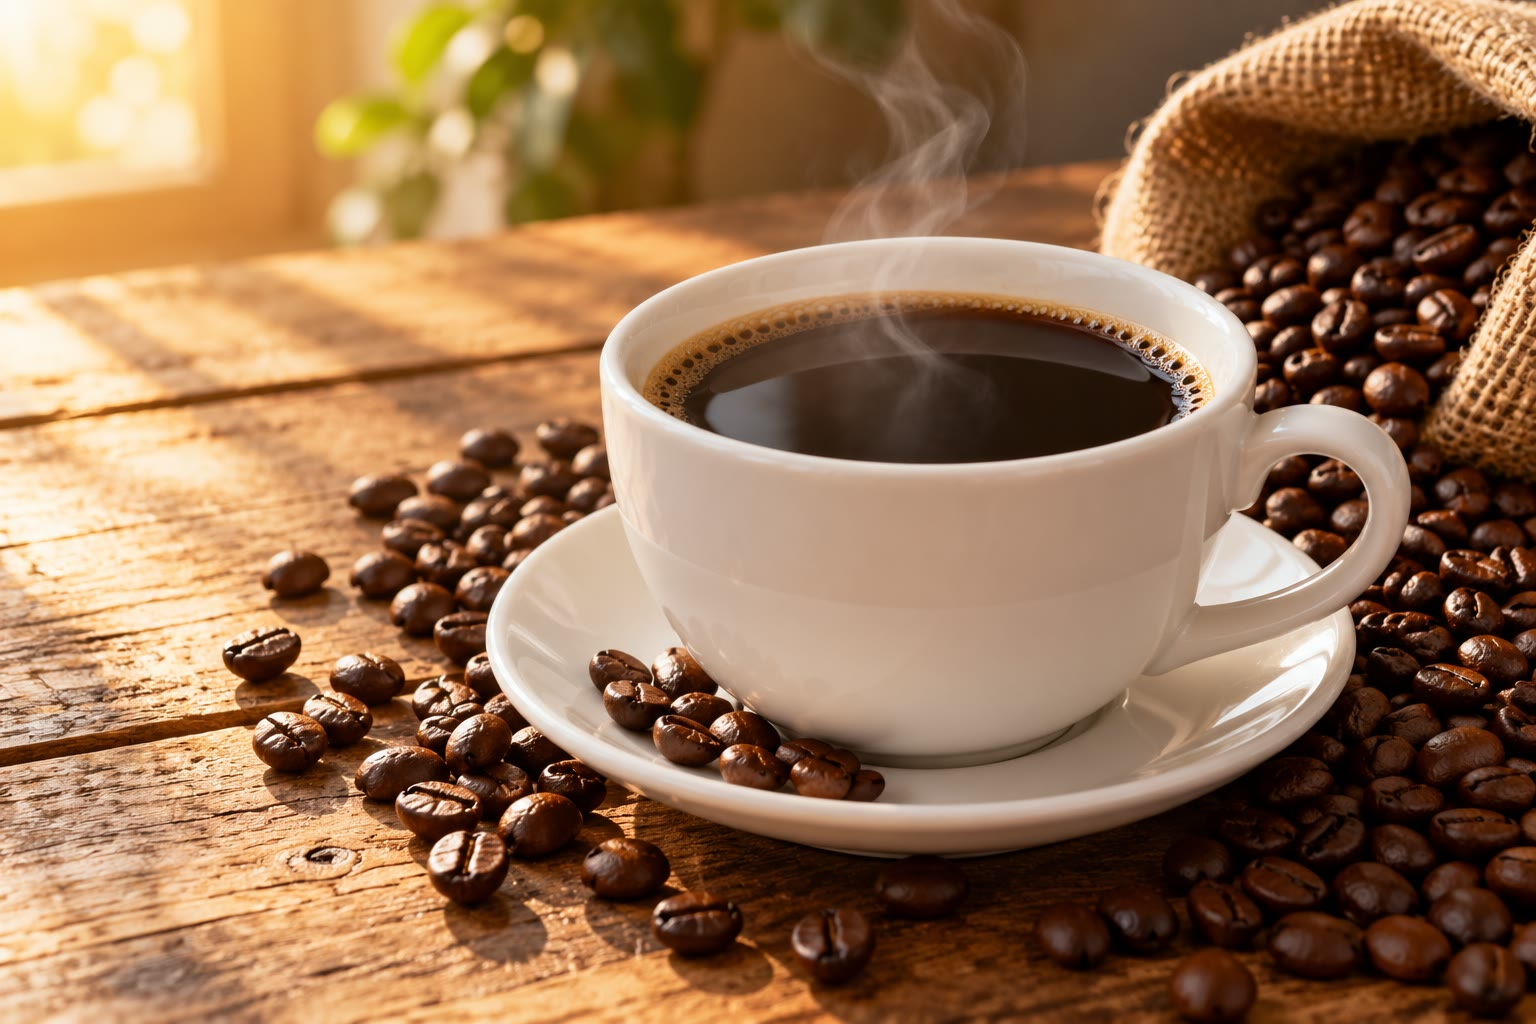
\includegraphics[width=0.5\linewidth]{images/book4/ai/b3-29-coffee.jpg}

{\small فنجان قهوة وحبوب محمّصة: الكافيين، وهو بيورين، وكثير من
جزيئات الرائحة المتكوّنة في التحميص \omterm{def:b3:heterocycles:heterocycle}{حلقات غير متجانسة}.}
\end{omfigure}

\section{الحلقات العطرية غير المتجانسة}

\begin{definition}[الحلقات غير المتجانسة]\label{def:b3:heterocycles:heterocycle}
\emph{المركب الحلقي غير المتجانس}\index{مركب حلقي غير متجانس} مركب حلقي فيه ذرة واحدة
على الأقل غير الكربون في الحلقة؛ و\emph{المركب العطري غير
المتجانس}\index{مركب عطري غير متجانس} مركب حلقي غير متجانس عطري، مثل البيريدين،
والبيرول، والفيوران أو الثيوفين.
\end{definition}

\begin{proposition}[ستة إلكترونات $\pi$]\label{prop:b3:heterocycles:sextet}
لكل من البيريدين والبيرول والفيوران والثيوفين والإيميدازول ستة إلكترونات $\pi$ في
حلقة مستوية حلقية مترافقة، وهي عطرية بحسب قاعدة هوكل.
\end{proposition}

\begin{proof}
البيريدين: تعطي ذرات الكربون الخمس والنيتروجين إلكترون p واحدًا لكل منها؛ ويقع الزوج
الحر للنيتروجين في مدار $sp^2$ في مستوي الحلقة، خارج النظام $\pi$: $5 + 1 = 6$.
البيرول: تعطي ذرات الكربون الأربع واحدًا لكل منها، والنيتروجين، المرتبط بالهيدروجين في المستوي،
يضع زوجه الحر في مداره p: $4 + 2 = 6$. الفيوران والثيوفين: كالبيرول، إذ
تعطي الذرة غير المتجانسة أحد زوجيها الحرين (ويقع الآخر في المستوي). الإيميدازول:
يعطي نيتروجين N--H اثنين، والنيتروجين الشبيه بنيتروجين البيريدين واحدًا، وذرات الكربون الثلاث
ثلاثة: 6. والعدد ستة هو $4n + 2$ مع $n = 1$.
\end{proof}

\begin{omfigure}
\begin{tikzpicture}[font=\small, yscale=0.55]
  % pyridine: six p orbitals perpendicular to the ring (drawn first), N at 0 deg
  \foreach \a in {0,60,...,300} { \pic at (\a:1.1) {omp={0.62}{90}}; }
  \draw[thick] (0:1.1) -- (60:1.1) -- (120:1.1) -- (180:1.1) -- (240:1.1) -- (300:1.1) -- cycle;
  \node[fill=white, inner sep=0.5pt] at (0:1.1) {N};
  \pic at ($(0:1.1)+(0.2,0)$) {omlobe={0.8}{0}};
  \node[font=\scriptsize, align=center, anchor=north] at (0,-2.4) {\foreignlanguage{arabic}{البيريدين: 6 إلكترونات p من 6 ذرات؛}\\ \foreignlanguage{arabic}{زوج حر في المستوي، فهو قاعدي}};
  \begin{scope}[xshift=5.4cm]
    \foreach \a in {0,72,144,216,288} { \pic at (\a:1.0) {omp={0.62}{90}}; }
    \draw[thick] (0:1.0) -- (72:1.0) -- (144:1.0) -- (216:1.0) -- (288:1.0) -- cycle;
    \node[fill=white, inner sep=0.5pt] at (0:1.0) {N};
    \draw ($(0:1.0)+(0.18,0)$) -- (0:1.7) node[right, inner sep=0.5pt] {H};
    \node[font=\scriptsize, align=center, anchor=north] at (0,-2.4) {\foreignlanguage{arabic}{البيرول: الزوج الحر للذرة N أحد}\\ \foreignlanguage{arabic}{إلكترونات $\pi$ الستة، فهو غير قاعدي}};
  \end{scope}
\end{tikzpicture}

{\small النظامان $\pi$ للبيريدين والبيرول، منظورًا إليهما بميل: مدار p واحد لكل
ذرة في الحلقة، عمودي على الحلقة. في البيريدين يتجه الزوج الحر للنيتروجين (الفص الواقع في المستوي، عند
النيتروجين) إلى الخارج في مستوي الحلقة وهو حر في ربط بروتون؛ أما في البيرول فإن
النيتروجين، الذي يحمل هيدروجينًا في المستوي، يعطي زوجه الحر للسداسية
العطرية.}
\end{omfigure}

\begin{definition}[الحلقات غير المتجانسة الفائضة $\pi$ والناقصة $\pi$]\label{def:b3:heterocycles:pi-character}
\emph{الحلقة غير المتجانسة الفائضة $\pi$}\index{حلقة غير متجانسة فائضة باي@حلقة غير متجانسة فائضة $\pi$}، مثل
البيرول أو الفيوران أو الثيوفين، فيها ستة إلكترونات $\pi$ على خمس ذرات وكثافة
إلكترونات $\pi$ على ذرات كربونها أعلى منها في البنزين؛ و\emph{الحلقة غير المتجانسة الناقصة
$\pi$}\index{حلقة غير متجانسة ناقصة باي@حلقة غير متجانسة ناقصة $\pi$}، مثل البيريدين، فيها
ذرة كهرسلبية في الحلقة تسحب كثافة $\pi$ من ذرات الكربون.
\end{definition}

\begin{proposition}[القاعدية]\label{prop:b3:heterocycles:basicity}
البيريدين قاعدة متوسطة والبيرول لا يكاد يكون قاعدة؛ والبيرول، حين
يُبرتن في حمض قوي، يأخذ البروتون على الكربون، لا على النيتروجين.
\end{proposition}

\begin{proof}[تعليل]
% ledger: pka:pyridinium, pka4:pyrrolium, pka4:piperidinium, pka4:imidazolium, pka4:DMAPH
يقع الزوج الحر للبيريدين خارج النظام $\pi$: فبرتنته لا تكلّف شيئًا من
العطرية، وللبيريدينيوم $\mathrm pK_a = 5.2$؛ وهو أقل قاعدية من البيبيريدين
(فنيتروجين البيريدينيوم $sp^2$، أكثر طابعًا s، فيمسك زوجه
بقوة أكبر: البيبيريدينيوم 11.1). وبرتنة نيتروجين البيرول كانت ستُخرج زوجه
الحر من السداسية وتُتلف العطرية؛ ولا تبرتن البيرول إطلاقًا إلا الأحماض القوية جدًا،
وعند C2، حيث يحتفظ الكاتيون بشيء من الانتشار
($\mathrm pK_a$ نحو $-4$). وللإيميدازول نوعا النيتروجين كلاهما: فيُبرتن على
النيتروجين الشبيه بنيتروجين البيريدين، ويستقر كاتيونه المتناظر بالرنين ($\mathrm pK_a$
7.0)، ولهذا يعمل الهستيدين حمضًا وقاعدة في الإنزيمات.
و4-(ثنائي ميثيل أمينو)بيريدين أكثر قاعدية أيضًا ($\mathrm pK_a$ 9.6): فمجموعة الأمينو تدفع
زوجها الحر في الحلقة نحو نيتروجين الحلقة.
\end{proof}

% ledger: dip:pyridine, dip4:pyrrole, dip4:furan, dip4:thiophene
تحكي عزوم ثنائي القطب القصة نفسها: فللبيريدين (\qty{2.19}{D}) طرفه السالب
على النيتروجين، بينما في البيرول (\qty{1.84}{D}) يضع التبرع بالزوج الحر للحلقة
الطرفَ السالب على الحلقة والموجبَ على النيتروجين. وفي الفيوران
(\qty{0.66}{D}) والثيوفين (\qty{0.55}{D}) يكاد الأثران، السحب $\sigma$ والتبرع $\pi$،
يتلاشيان.

\begin{omfigure}
% ledger: h1:pyridine.a, h1:pyridine.g, h1:pyridine.b, h1:pyrrole.a, h1:pyrrole.b, h1:pyrrole.NH, h1:furan.a, h1:furan.b
\begin{tikzpicture}
\begin{axis}[width=0.86\linewidth, height=6.2cm, x dir=reverse, xmin=5.8, xmax=9.0, ymin=-0.1, ymax=3.6,
  axis x line=bottom, axis y line=none, xlabel={\babelsublr{$\delta$ / ppm}}, tick label style={font=\scriptsize}, label style={font=\small}]
\addplot[omDef, thick] table[x=ppm, y expr=\thisrow{y}+2.4] {figdata/out/bachelor-3-heterocycle-nmr-pyridine.dat};
\addplot[omThm, thick] table[x=ppm, y expr=\thisrow{y}+1.2] {figdata/out/bachelor-3-heterocycle-nmr-pyrrole.dat};
\addplot[omMeth, thick] table[x=ppm, y=y] {figdata/out/bachelor-3-heterocycle-nmr-furan.dat};
\node[font=\scriptsize, omDef, anchor=west] at (axis cs:7.1,3.0) {\foreignlanguage{arabic}{البيريدين: \babelsublr{H2/6, H4, H3/5 (2\,:\,1\,:\,2)}}};
\node[font=\scriptsize, omThm, anchor=west] at (axis cs:7.7,1.8) {\foreignlanguage{arabic}{البيرول: \babelsublr{NH, H2/5, H3/4}}};
\node[font=\scriptsize, omMeth, anchor=west] at (axis cs:7.2,0.6) {\foreignlanguage{arabic}{الفيوران: \babelsublr{H2/5, H3/4}}};
\end{axis}
\end{tikzpicture}

{\small الرنين المغناطيسي النووي البروتوني للبيريدين والبيرول والفيوران في الكلوروفورم المدوتر،
مركَّب من الانزياحات المقيسة في صورة خطوط مفردة (مع إهمال الاقترانات)، 
ومساحاتها تساوي أعداد البروتونات. للبيريدين الناقص $\pi$ إشارتا H2/6 وH4
في المجال المنخفض بعيدًا عن إشارة البنزين؛ أما البيرول والفيوران الفائضان $\pi$ فمعظم
إشاراتهما في المجال المرتفع منها؛ والبروتونات المجاورة للذرة غير المتجانسة هي دائمًا الأقل
حجبًا.}
\end{omfigure}

\section{البيريدين}

يقاوم البيريدين الاستبدال المحب للإلكترونات: فالمحب للإلكترونات يلاقي حلقة
أفقر بالإلكترونات من البنزين، وفي الحمض الموجود عادةً، أيون
بيريدينيوم تصده شحنته الموجبة. وتحتاج النترتة إلى ظروف
قاسية جدًا وتعطي المتماكب 3 بمردود ضعيف.

\begin{proposition}[الاستبدال المحب للإلكترونات عند C3]\label{prop:b3:heterocycles:pyridine-c3}
يحدث الهجوم المحب للإلكترونات على البيريدين عند C3: فالهجوم عند C2 أو C4 يعطي
وسيط ويلاند تضع إحدى بنياته الرنينية الشحنة الموجبة
على نيتروجين لا يحيط به إلا ستة إلكترونات.
\end{proposition}

\begin{proof}
في الكاتيون الناتج عن الهجوم عند C2 (أو C4) تنتشر الشحنة الموجبة على C3 وC5
وN1 (أو C3 وC5 وN1): بنية رنينية فيها نيتروجين فقير بالإلكترونات
سداسي الإلكترونات، وهذا غير ملائم جدًا لذرة كهرسلبية. أما الهجوم
عند C3 فينشر الشحنة على C2 وC4 وC6 فقط. والكاتيونات الثلاثة كلها أقل استقرارًا
من كاتيون البنزين، لكن الهجوم عند C3 هو الأقل سوءًا.
\end{proof}

\begin{definition}[N-أكسيد البيريدين]\label{def:b3:heterocycles:n-oxide}
\emph{N-أكسيد البيريدين}\index{N-أكسيد البيريدين}، المصنوع بأكسدة البيريدين
بحمض بيروكسي، فيه مجموعة $\mathrm{N^+{-}O^-}$ يعيد أكسجينها إلكترونات إلى C2
وC4؛ فيخضع للاستبدال المحب للإلكترونات عند C4، ثم يُنزع
الأكسجين.
\end{definition}

\begin{definition}[الاستبدال العطري المحب للنواة]\label{def:b3:heterocycles:snar}
\emph{الاستبدال العطري المحب للنواة}\index{استبدال عطري محب للنواة}
($\mathrm S_\mathrm NAr$) يستبدل بمجموعة مغادرة على حلقة عطرية فقيرة بالإلكترونات
محبًّا للنواة، عبر إضافة يليها حذف. ووسيط الإضافة
الأنيوني هو \emph{معقد مايزنهايمر}\index{معقد مايزنهايمر}.
\end{definition}

\begin{proposition}[$\mathrm S_\mathrm NAr$ عند C2 وC4]\label{prop:b3:heterocycles:snar-positions}
تخضع هالوبيريدينات للتفاعل $\mathrm S_\mathrm NAr$ بسهولة عند C2 وC4 وببطء شديد فقط عند C3،
لأن الإضافة عند C2 أو C4 تضع الشحنة السالبة على النيتروجين.
\end{proposition}

\begin{proof}
الإضافة عند C2 تجعل C2 من نوع $sp^3$ وتترك أربعة إلكترونات $\pi$ مع الزوج القادم
منتشرة على N1 وC3 وC5 (أو من أجل C4: C3 وC5 وN1): فإحدى البنى الرنينية تضع
الشحنة السالبة على النيتروجين الكهرسلبي. أما الإضافة عند C3 فتنشرها على
C2 وC4 وC6 فقط، وكلها ذرات كربون.
\end{proof}

\begin{omfigure}
\begin{tikzpicture}[font=\small, >=Stealth]
  \draw[thick] (-0.000,-0.620) -- (0.537,-0.310) -- (0.537,0.310) -- (0.000,0.620) -- (-0.537,0.310) -- (-0.537,-0.310) -- cycle;
  \draw[thick] (0.082,-0.424) -- (0.326,-0.283);
  \draw[thick] (0.326,0.283) -- (0.082,0.424);
  \draw[thick] (-0.408,0.141) -- (-0.408,-0.141);
  \node[fill=white, inner sep=0.4pt, font=\scriptsize] at (-0.000,-0.620) {N};
  \draw (0.537,-0.310) -- (0.927,-0.535) node[right, inner sep=0.5pt, font=\scriptsize] {Cl};
  \draw[thick] (3.400,-0.620) -- (3.937,-0.310) -- (3.937,0.310) -- (3.400,0.620) -- (2.863,0.310) -- (2.863,-0.310) -- cycle;
  \draw[thick] (3.726,0.283) -- (3.482,0.424);
  \draw[thick] (2.992,0.141) -- (2.992,-0.141);
  \node[fill=white, inner sep=0.4pt, font=\scriptsize] at (3.400,-0.620) {N};
  \node[font=\scriptsize, omThm] at (3.350,-0.920) {$\ominus$};
  \draw (3.937,-0.310) -- (4.386,-0.343) node[right, inner sep=0.5pt, font=\scriptsize] {Nu};
  \draw (3.937,-0.310) -- (4.190,-0.682) node[right, inner sep=0.5pt, font=\scriptsize] {Cl};
  \draw[thick] (6.800,-0.620) -- (7.337,-0.310) -- (7.337,0.310) -- (6.800,0.620) -- (6.263,0.310) -- (6.263,-0.310) -- cycle;
  \draw[thick] (6.882,-0.424) -- (7.126,-0.283);
  \draw[thick] (7.126,0.283) -- (6.882,0.424);
  \draw[thick] (6.392,0.141) -- (6.392,-0.141);
  \node[fill=white, inner sep=0.4pt, font=\scriptsize] at (6.800,-0.620) {N};
  \draw (7.337,-0.310) -- (7.727,-0.535) node[right, inner sep=0.5pt, font=\scriptsize] {Nu};
  \draw[->, thick] (1.25,0) -- (2.35,0) node[midway, above, font=\scriptsize] {$+\,\mathrm{Nu^-}$};
  \draw[->, thick] (4.65,0) -- (5.75,0) node[midway, above, font=\scriptsize] {$-\,\ce{Cl-}$};
  \node[font=\scriptsize] at (3.4,-1.2) {\foreignlanguage{arabic}{معقد مايزنهايمر}};
\end{tikzpicture}

{\small الاستبدال المحب للنواة في 2-كلوروبيريدين: يُضاف المحب للنواة إلى
C2، فيعطي وسيطًا أنيونيًا تقع شحنته السالبة أساسًا على
نيتروجين الحلقة (بنية رنينية واحدة معروضة)؛ ثم يغادر الكلوريد وتُستعاد
الحلقة العطرية.}
\end{omfigure}

\begin{proposition}[الإضافة--الحذف]\label{prop:b3:heterocycles:snar-mechanism}
من أجل تفاعل $\mathrm S_\mathrm NAr$ تكون خطوة إضافته هي المحددة للسرعة، $v = k[\mathrm{ArX}][\mathrm{Nu^-}]$،
ويكون الفلوريد أفضل الهاليدات مجموعةً مغادرة.
\end{proposition}

\begin{proof}[تعليل]
السرعة هي سرعة الإضافة الثنائية الجزيئية. ولا تنكسر الرابطة كربون--هالوجين
في تلك الخطوة؛ والمهم هو مقدار ما يخفضه الهالوجين من طاقة
الحالة الانتقالية الأنيونية بسحبه الإلكترونات، والفلور، الأكثر
كهرسلبية، يفعل ذلك أكثر: فالترتيب F $>$ Cl $\approx$ Br $>$ I، عكس ترتيب $\mathrm S_\mathrm N2$.
\end{proof}

\begin{definition}[تفاعل تشيتشيبابين]\label{def:b3:heterocycles:chichibabin}
\emph{تفاعل تشيتشيبابين}\index{تفاعل تشيتشيبابين} هو أمينة
البيريدين عند C2 بأميد الصوديوم: يُضاف أيون الأميد إلى C2، ويُفقد أيون هيدريد،
في صورة ثنائي الهيدروجين بعد تفاعله مع الناتج.
\end{definition}

يعمل البيريدين وDMAP أيضًا قاعدتين وحفازين محبين للنواة: ففي
الأسيلات بأنهيدريدات الأحماض، يهاجم DMAP الأنهيدريد أولًا، فيعطي
أيون أسيل بيريدينيوم ينقل مجموعة الأسيل إلى الكحول أسرع بكثير من
الأنهيدريد نفسه. والبيريدينات وثنائيات البيريدين والفينانترولينات من بين
أكثر ربائط كيمياء التناسق شيوعًا.

\section{الحلقات الخماسية}

\begin{proposition}[الاستبدال المحب للإلكترونات في البيرول عند C2]\label{prop:b3:heterocycles:pyrrole-c2}
يخضع البيرول والفيوران والثيوفين للاستبدال المحب للإلكترونات أساسًا عند C2،
لأن للكاتيون الناتج عن الهجوم عند C2 ثلاث بنى رنينية وللكاتيون
الناتج عن الهجوم عند C3 بنيتين فقط.
\end{proposition}

\begin{proof}
بعد الهجوم عند C2، يمكن أن تقع الشحنة الموجبة على C3، أو على C5، أو على النيتروجين،
حيث تُتقاسم عبر الزوج الحر وتحتفظ كل ذرة بثمانيتها (البنية
الثالثة). وبعد الهجوم عند C3، لا يمكن أن تقع إلا على C2 أو على النيتروجين: فتكون الشحنة
أقل انتشارًا (انظر الشكل).
\end{proof}

\begin{omfigure}
\begin{tikzpicture}[font=\small]
  \draw[thick] (0.000,0.620) -- (0.590,0.192) -- (0.364,-0.502) -- (-0.364,-0.502) -- (-0.590,0.192) -- cycle;
  \draw[thick] (-0.303,-0.269) -- (-0.403,0.039);
  \node[fill=white, inner sep=0.4pt, font=\scriptsize] at (0.000,0.620) {N};
  \draw (0.000,0.750) -- (0.000,1.020) node[above, inner sep=0.5pt, font=\scriptsize] {H};
  \draw (0.590,0.192) -- (0.893,0.482) node[right, inner sep=0.5pt, font=\scriptsize] {H};
  \draw (0.590,0.192) -- (1.006,0.135) node[right, inner sep=0.5pt, font=\scriptsize] {E};
  \node[font=\scriptsize, omThm] at (0.164,-0.226) {$\oplus$};
  \draw[thick] (2.600,0.620) -- (3.190,0.192) -- (2.964,-0.502) -- (2.236,-0.502) -- (2.010,0.192) -- cycle;
  \draw[thick] (2.762,-0.371) -- (2.438,-0.371);
  \node[fill=white, inner sep=0.4pt, font=\scriptsize] at (2.600,0.620) {N};
  \draw (2.600,0.750) -- (2.600,1.020) node[above, inner sep=0.5pt, font=\scriptsize] {H};
  \draw (3.190,0.192) -- (3.493,0.482) node[right, inner sep=0.5pt, font=\scriptsize] {H};
  \draw (3.190,0.192) -- (3.606,0.135) node[right, inner sep=0.5pt, font=\scriptsize] {E};
  \node[font=\scriptsize, omThm] at (2.335,0.086) {$\oplus$};
  \draw[thick] (5.200,0.620) -- (5.790,0.192) -- (5.564,-0.502) -- (4.836,-0.502) -- (4.610,0.192) -- cycle;
  \draw[thick] (5.362,-0.371) -- (5.038,-0.371);
  \draw[thick] (5.113,0.395) -- (4.851,0.205);
  \node[fill=white, inner sep=0.4pt, font=\scriptsize] at (5.200,0.620) {N};
  \draw (5.200,0.750) -- (5.200,1.020) node[above, inner sep=0.5pt, font=\scriptsize] {H};
  \draw (5.790,0.192) -- (6.093,0.482) node[right, inner sep=0.5pt, font=\scriptsize] {H};
  \draw (5.790,0.192) -- (6.206,0.135) node[right, inner sep=0.5pt, font=\scriptsize] {E};
  \node[font=\scriptsize, omThm] at (5.480,0.700) {$\oplus$};
  \draw[thick] (8.400,0.620) -- (8.990,0.192) -- (8.764,-0.502) -- (8.036,-0.502) -- (7.810,0.192) -- cycle;
  \draw[thick] (8.097,-0.269) -- (7.997,0.039);
  \node[fill=white, inner sep=0.4pt, font=\scriptsize] at (8.400,0.620) {N};
  \draw (8.400,0.750) -- (8.400,1.020) node[above, inner sep=0.5pt, font=\scriptsize] {H};
  \draw (8.764,-0.502) -- (9.135,-0.700) node[right, inner sep=0.5pt, font=\scriptsize] {H};
  \draw (8.764,-0.502) -- (8.839,-0.915) node[right, inner sep=0.5pt, font=\scriptsize] {E};
  \node[font=\scriptsize, omThm] at (8.665,0.086) {$\oplus$};
  \draw[thick] (11.000,0.620) -- (11.590,0.192) -- (11.364,-0.502) -- (10.636,-0.502) -- (10.410,0.192) -- cycle;
  \draw[thick] (10.697,-0.269) -- (10.597,0.039);
  \draw[thick] (11.087,0.395) -- (11.349,0.205);
  \node[fill=white, inner sep=0.4pt, font=\scriptsize] at (11.000,0.620) {N};
  \draw (11.000,0.750) -- (11.000,1.020) node[above, inner sep=0.5pt, font=\scriptsize] {H};
  \draw (11.364,-0.502) -- (11.735,-0.700) node[right, inner sep=0.5pt, font=\scriptsize] {H};
  \draw (11.364,-0.502) -- (11.439,-0.915) node[right, inner sep=0.5pt, font=\scriptsize] {E};
  \node[font=\scriptsize, omThm] at (11.280,0.700) {$\oplus$};
  \node[font=\scriptsize] at (2.6,-1.35) {\foreignlanguage{arabic}{الهجوم عند \babelsublr{C2}: ثلاث بنى}};
  \node[font=\scriptsize] at (9.7,-1.35) {\foreignlanguage{arabic}{الهجوم عند \babelsublr{C3}: بنيتان}};
  \draw[black!40] (6.8,-1.2) -- (6.8,1.2);
\end{tikzpicture}

{\small وسائط ويلاند للبيرول (E: المحب للإلكترونات؛ $\oplus$: الشحنة الموجبة).
يعطي الهجوم عند C2 كاتيونًا تقع شحنته على C3، أو على C5، أو على النيتروجين مع اكتمال كل
الثمانيات؛ والهجوم عند C3، على C2 أو النيتروجين فقط.}
\end{omfigure}

البيرول بتفاعلية الفينول أو الأنيلين تقريبًا: فهو يُبرمَن ويُنترَت
ويُؤسيَل في ظروف معتدلة، ويتبلمر في الحمض القوي، 
ويُفرمَل عند C2 بكاشف فيلسماير المصنوع من ثنائي ميثيل فورماميد وكلوريد
الفوسفوريل. وتتناقص التفاعليات بالترتيب البيرول $>$ الفيوران $>$ الثيوفين $>$ البنزين،
تبعًا لاستعداد الذرة غير المتجانسة لمشاركة زوجها الحر. والفيوران،
الأقل عطرية، يتفاعل أيضًا ديينًا في تفاعلات ديلز--ألدر. والقواعد
القوية مثل البيوتيل ليثيوم تنزع بروتون الفيوران والثيوفين عند C2، بجوار
الذرة غير المتجانسة، فتعطي كواشف ليثيوم عضوية.

\begin{method}[التنبؤ بموضع الهجوم على حلقة غير متجانسة]\label{met:b3:heterocycles:site}
\begin{enumerate}
  \item صنّف الحلقة: فائضة $\pi$ (ذرة غير متجانسة شبيهة بنيتروجين البيرول) أو ناقصة $\pi$
        (نيتروجين شبيه بنيتروجين البيريدين).
  \item المحبات للإلكترونات: على حلقة فائضة $\pi$ عند C2 (وعند C3 في الإندول، الذي كان الهجوم عند C2 فيه
        سيخل بحلقة البنزين)؛ وعلى البيريدين عند C3، أو عند C4 عبر
        N-أكسيده.
  \item المحبات للنواة: على حلقة ناقصة $\pi$ عند C2 أو C4، خاصة مع مجموعة
        مغادرة هناك.
  \item القواعد القوية: عند الرابطة C--H المجاورة للذرة غير المتجانسة.
\end{enumerate}
\end{method}

\section{الحلقات غير المتجانسة الملتحمة والحيوية}

يتفاعل الإندول، وهو بنزين ملتحم ببيرول، مع المحبات للإلكترونات عند C3: فهناك
يحتفظ الوسيط بحلقة البنزين سليمة، مع الشحنة على النيتروجين.
ويُستبدل الكينولين، وهو بنزين ملتحم ببيريدين، بالمحبات للإلكترونات على
حلقة البنزين فيه وبالمحبات للنواة عند C2 وC4. والقواعد النووية
بيريميدينات (السيتوزين، والثايمين، واليوراسيل) وبيورينات (الأدينين، والغوانين)، أي
بيريميدين ملتحم بإيميدازول. وصورها الأوكسو والأمينو (المتصاوغات اللاكتامية
والأمينية) تغلب على صورها الهيدروكسي والإيمينو، وهذا يثبّت نمط
المانحات والمستقبلات للروابط الهيدروجينية على كل قاعدة، ومنه تزاوج القواعد.

\begin{omfigure}
\begin{tikzpicture}[font=\small]
  \node[draw, rounded corners, minimum width=1.8cm, minimum height=2.8cm, fill=omDef!8] at (0,0) {};
  \node[font=\small\bfseries] at (0,1.75) {\foreignlanguage{arabic}{الغوانين}};
  \node[anchor=east] (g1) at (0.85,0.85) {C6=O};
  \node[anchor=east] (g2) at (0.85,0) {N1--H};
  \node[anchor=east] (g3) at (0.85,-0.85) {C2--N--H};
  \node[draw, rounded corners, minimum width=1.8cm, minimum height=2.8cm, fill=omThm!8] at (3.2,0) {};
  \node[font=\small\bfseries] at (3.2,1.75) {\foreignlanguage{arabic}{السيتوزين}};
  \node[anchor=west] (c1) at (2.35,0.85) {H--N--C4};
  \node[anchor=west] (c2) at (2.35,0) {N3};
  \node[anchor=west] (c3) at (2.35,-0.85) {O=C2};
  \draw[omMeth, very thick, dotted] (g1.east) -- (c1.west);
  \draw[omMeth, very thick, dotted] (g2.east) -- (c2.west);
  \draw[omMeth, very thick, dotted] (g3.east) -- (c3.west);
\end{tikzpicture}

{\small زوج القاعدتين غوانين--سيتوزين، رسم تخطيطي: ثلاث روابط هيدروجينية (بالأخضر)
بين أكسجين كربونيل الغوانين ورابطة N--H أمينية في السيتوزين، وبين N1--H في
الغوانين وN3 في حلقة السيتوزين، وبين رابطة N--H أمينية في الغوانين 
وأكسجين كربونيل السيتوزين. ويكوّن الأدينين والثايمين رابطتين.}
\end{omfigure}

\section{بناء الحلقات}

\begin{definition}[تخليق بال--كنور]\label{def:b3:heterocycles:paal-knorr}
\emph{تخليق بال--كنور}\index{تخليق بال--كنور} يصنع فيورانًا
(بالحمض)، أو بيرولًا (بأمين أولي أو بالأمونيا) أو ثيوفينًا (بكاشف
كبريتي) من مركب ثنائي الكربونيل 1،4.
\end{definition}

\begin{definition}[تخليق هانتش للبيريدين]\label{def:b3:heterocycles:hantzsch}
\emph{تخليق هانتش للبيريدين}\index{تخليق هانتش للبيريدين}
يكثّف ألدهيدًا ومكافئين من إستر $\beta$-كيتوني والأمونيا في
1،4-ثنائي هيدروبيريدين، يمكن أن يتأكسد إلى البيريدين.
\end{definition}

\begin{definition}[تخليق فيشر للإندول]\label{def:b3:heterocycles:fischer-indole}
\emph{تخليق فيشر للإندول}\index{تخليق فيشر للإندول} يسخّن
فينيل هيدرازون ألدهيد أو كيتون مع حفاز حمضي: يتصاوغ الهيدرازون
إلى إين-هيدرازين، يخضع \omterm{def:b3:pericyclic:families}{لإعادة ترتيب سيغماتروبية} [3,3]؛
ثم يعطي التحلّق وفقد الأمونيا الإندول.
\end{definition}

\begin{omfigure}
\setchemfig{atom sep=1.8em}
\schemestart
\chemfig{*6(-=-=(-NH-[:30]N=[:-30](-[:-90]CH_3)-[:30]CH_3)-=)}
\arrow{->[$\ce{H+}$][تصاوغ]}[,1.4]
\chemfig{*6(-=-=(-NH-[:30]NH-[:-30](=[:-90]CH_2)-[:30]CH_3)-=)}
\schemestop
\par\bigskip
\schemestart
\arrow{->[{[3,3]}، ثم][تحلّق، $-\ce{NH3}$]}[,2.2]
\chemfig{*6(-=*5(-=(-CH_3)-N(-H)-)-=-=)}
\schemestop

{\small \omterm{def:b3:heterocycles:fischer-indole}{تخليق فيشر للإندول} من فينيل هيدرازون الأسيتون. يحوّل الحمض
الهيدرازون إلى متصاوغه الإين-هيدرازيني؛ وتكسر إعادة الترتيب [3,3] الرابطة
N--N وتكوّن رابطة C--C بين كربون الحلقة الواقع في الموضع \textit{ortho} من النيتروجين 
ومجموعة $\ce{CH2}$ الطرفية؛ ثم يهاجم الأمين الجديد الإيمين، ويعطي فقد الأمونيا
2-ميثيل إندول.}
\end{omfigure}

\begin{method}[فصل حلقة غير متجانسة]\label{met:b3:heterocycles:disconnect}
\begin{enumerate}
  \item بيرول أو فيوران أو ثيوفين ثنائي الاستبدال 2،5: افصل الرابطتين المتصلتين
        بالذرة غير المتجانسة، رجوعًا إلى ثنائي كيتون 1،4 (بال--كنور).
  \item 1،4-ثنائي هيدروبيريدين متناظر بإسترين عند C3 وC5: رجوعًا إلى
        ألدهيد واحد، وإستري $\beta$-كيتونيين والأمونيا (هانتش).
  \item إندول ثنائي الاستبدال 2،3: رجوعًا إلى فينيل هيدرازين والكيتون
        $\mathrm{R^2CH_2COR^3}$ (فيشر).
  \item تحقّق من توفر القطع، ثم من الانتقائية الموضعية حين يكون الكيتون
        غير متناظر.
\end{enumerate}
\end{method}

\begin{definition}[المماثل الحيوي]\label{def:b3:heterocycles:bioisostere}
\emph{المماثل الحيوي}\index{مماثل حيوي} مجموعة تحل محل أخرى في
جزيء دواء مع الحفاظ على نشاطه الحيوي، لأن لها حجمًا وشكلًا
ونمطًا من الروابط الهيدروجينية والشحنة متشابهة، مثل التترازول
مكان الحمض الكربوكسيلي، أو البيريدين مكان حلقة البنزين.
\end{definition}

\begin{inthelab}[بيرول بال--كنور]
يُسخَّن هكسان-2،5-ديون والأنيلين وكمية حفزية من حمض 4-تولوين سلفونيك
مع التقطير الارتدادي في التولوين في دورق مزود بمصيدة دين--ستارك: فيُحمل
الماء المتكوّن في صورة أزيوتروب ويتجمع في الذراع الجانبية، وهذا
يدفع التكاثف حتى الاكتمال. وحين لا ينفصل مزيد من الماء، يُغسل
المحلول بمحلول مائي من هيدروجين كربونات الصوديوم، ويُجفف ويُبخَّر،
ويُعاد تبلير 2،5-ثنائي ميثيل-1-فينيل بيرول.
\end{inthelab}

\begin{safety}{\ghs[0.62cm]{GHS02}\ghs[0.62cm]{GHS06}\ghs[0.62cm]{GHS07}\ghs[0.62cm]{GHS08}\ghs[0.62cm]{GHS09}}
% ledger: ghs4:pyridine, ghs4:phenylhydrazine
البيريدين: شديد الاشتعال، ضار بكل طرق التعرض، ذو رائحة قوية؛ يُستعمل تحت
ساحبة الأبخرة. الفينيل هيدرازين: سام بكل طرق التعرض، قد يسبب السرطان والعيوب
الوراثية، ويُتلف الدم عند التعرض المتكرر، ومحسِّس، وشديد السمية
للأحياء المائية؛ يوزن تحت ساحبة الأبخرة بالقفازات، وتُجمع نفاياته
على حدة.
\end{safety}

\begin{history}[تخليقان كلاسيكيان للحلقات]
وصف إميل فيشر تخليقه للإندول سنة 1883، في السنوات نفسها التي عمل فيها
على السكريات والبيورينات؛ ونشر آرثر هانتش تخليقه للبيريدين
سنة 1881. ولا يزال كلاهما مستعملًا: تخليق فيشر من أجل أدوية
التريبتان المضادة للشقيقة، وتخليق هانتش من أجل حاصرات قنوات الكالسيوم
من نوع ثنائي هيدروبيريدين التي تعالج ارتفاع ضغط الدم.
\end{history}

\section{تمارين}

\begin{exercise}[$\star$]\label{exo:b3:heterocycles:1}
عُدّ إلكترونات $\pi$ في الأوكسازول والثيازول والبيريميدين والبيورين، وقل أي
الأزواج الحرة تنتمي إلى النظام $\pi$.
\end{exercise}

\begin{exercise}[$\star$]\label{exo:b3:heterocycles:2}
رتّب البيريدين والبيرول والإيميدازول والبيبيريدين وDMAP بحسب القاعدية، مع
قيم $\mathrm pK_a$ لها.
\end{exercise}

\begin{exercise}[$\star$]\label{exo:b3:heterocycles:3}
أعطِ الناتج الرئيس للبرومة الأحادية للبيرول، وللفيوران، وللإندول.
\end{exercise}

\begin{exercise}[$\star$]\label{exo:b3:heterocycles:4}
أعطِ نواتج تفاعل بال--كنور للمركب هكسان-2،5-ديون مع الحمض وحده،
ومع ميثيل أمين، ومع خماسي كبريتيد الفوسفور.
\end{exercise}

\begin{exercise}[$\star\star$]\label{exo:b3:heterocycles:5}
يتفاعل 2-كلوروبيريدين مع ميثوكسيد الصوديوم في الميثانول عند \qty{65}{\celsius}؛ أما 3-كلوروبيريدين
فلا يكاد يتفاعل. فسّر، وأعطِ الناتج.
\end{exercise}

\begin{exercise}[$\star\star$]\label{exo:b3:heterocycles:6}
أعطِ ناتج \omterm{def:b3:heterocycles:chichibabin}{تفاعل تشيتشيبابين} للبيريدين وارسم وسيط
الإضافة.
\end{exercise}

\begin{exercise}[$\star\star$]\label{exo:b3:heterocycles:7}
يُنترَت \omterm{def:b3:heterocycles:n-oxide}{N-أكسيد البيريدين} عند C4. فسّر ذلك ببنى رنينية، وقل كيف
يُحصل على 4-نتروبيريدين.
\end{exercise}

\begin{exercise}[$\star\star$]\label{exo:b3:heterocycles:8}
يوجد 2-هيدروكسي بيريدين أساسًا في صورة 2-بيريدون في الماء. ارسم المتصاوغين 
وفسّر لماذا يبقى البيريدون عطريًا.
\end{exercise}

\begin{exercise}[$\star\star$]\label{exo:b3:heterocycles:9}
أعطِ مكوّنات تخليق هانتش للمركب 1،4-ثنائي هيدروبيريدين ذي
إستري الميثيل عند C3 وC5، ومجموعتي الميثيل عند C2 وC6 ومجموعة 2-نتروفينيل
عند C4.
\end{exercise}

\begin{exercise}[$\star\star\star$]\label{exo:b3:heterocycles:10}
يعطي البوتانون إندولين مختلفين في تخليق فيشر مع
الفينيل هيدرازين. أعطِ كليهما، وقل كيف تغيّر قوة الحمض نسبتهما.
\end{exercise}

\begin{exercise}[$\star\star\star$]\label{exo:b3:heterocycles:11}
فسّر لماذا يتفاعل 4-فلورونتروبنزين و2-فلوروبيريدين أسرع مع
المحبات للنواة من الكلوريدات الموافقة، خلافًا لركائز $\mathrm S_\mathrm N2$.
\end{exercise}

\begin{exercise}[$\star\star\star$]\label{exo:b3:heterocycles:12}
باستعمال الأطياف المركَّبة في الفصل، فسّر كيف تميّز البيريدين من
البيرول والفيوران بطيفها البروتوني، وتنبّأ بطيف
الثيوفين (الانزياحان \qty{7.33}{ppm} و\qty{7.12}{ppm}).
\end{exercise}

\section{مسألة: بناء إندول}

\begin{problem}[{مسألة نهاية الأسبوع --- بناء إندول: فينيل هيدرازون
الأسيتون، والإين-هيدرازين وإعادة ترتيبه [3,3]، وفقد الأمونيا،
والاختيار بين إندولين مع البوتانون}]
\label{pb:b3:heterocycles:1}
% ledger: aw:C, aw:H, aw:N, aw:O
معطيات المسألة: يتفاعل 10.0 g من الفينيل هيدرازين مع فائض من الأسيتون، 
ويُسخَّن الهيدرازون مع كلوريد الزنك.

\medskip\noindent\textbf{الجزء الأول --- الهيدرازون.}
\begin{enumerate}
  \item اكتب تكوّن فينيل هيدرازون الأسيتون.
  \item لماذا هو تكاثف من نمط تكوّن الإيمين، ولماذا يفيد أثر من الحمض؟
  \item أي ذرتي نيتروجين الفينيل هيدرازين تهاجم مجموعة الكربونيل، ولماذا؟
  \item احسب الكتلة المولية للفينيل هيدرازين والكمية المستعملة.
  \item احسب الكتلة النظرية للهيدرازون.
\end{enumerate}

\medskip\noindent\textbf{الجزء الثاني --- الإين-هيدرازين والخطوة [3,3].}
\begin{enumerate}[resume]
  \item ارسم المتصاوغ الإين-هيدرازيني.
  \item ما الذرات الست التي تكوّن الحالة الانتقالية الحلقية لإعادة الترتيب [3,3]؟
  \item أي رابطة تنكسر وأيها تتكوّن؟
  \item كم إلكترونًا يشارك، وهل الخطوة مسموحة حراريًا؟
  \item ماذا يفعل كلوريد الزنك؟
  \item لماذا يجب أن تُستعاد عطرية حلقة البنزين بعد ذلك؟
\end{enumerate}

\medskip\noindent\textbf{الجزء الثالث --- إغلاق الحلقة.}
\begin{enumerate}[resume]
  \item أي أمين يهاجم أي ذرة كربون ليغلق الحلقة الخماسية؟
  \item ما الجزيء الصغير الذي يغادر، وما الذي يدفع الخطوة الأخيرة؟
  \item اكتب المعادلة الإجمالية، من الهيدرازون إلى 2-ميثيل إندول.
  \item احسب الكتلة المولية للمركب 2-ميثيل إندول.
  \item احسب الكتلة النظرية للمركب 2-ميثيل إندول.
  \item أين يُستبدل 2-ميثيل إندول بمحب للإلكترونات، ولماذا؟
\end{enumerate}

\medskip\noindent\textbf{الجزء الرابع --- البوتانون.}
\begin{enumerate}[resume]
  \item ارسم الإين-هيدرازينين لفينيل هيدرازون البوتانون.
  \item أعطِ الإندولين اللذين يقودان إليهما.
  \item أي الإين-هيدرازينين أكثر استبدالًا، وأيهما يتكوّن في الحمض القوي؟
  \item أي إندول يغلب مع حمض ضعيف، ولماذا؟
  \item لماذا لا يستطيع فينيل هيدرازون الأسيتالدهيد أن يعطي الإندول نفسه جيدًا؟
  \item ماذا تعني مشكلة الانتقائية الموضعية لتخليق دواء؟
  \item اذكر النتيجة: الكتلة النظرية للمركب 2-ميثيل إندول من 10.0 g من
        الفينيل هيدرازين.
\end{enumerate}
\end{problem}
